\chapter{实验结果与分析}

在这一章中,本文将从质量和效率两方面来将本文提出的方法与前者的方法进行对比,并进行分析。

\section{质量对比}

\begin{figure*}[!t]
    \centering
    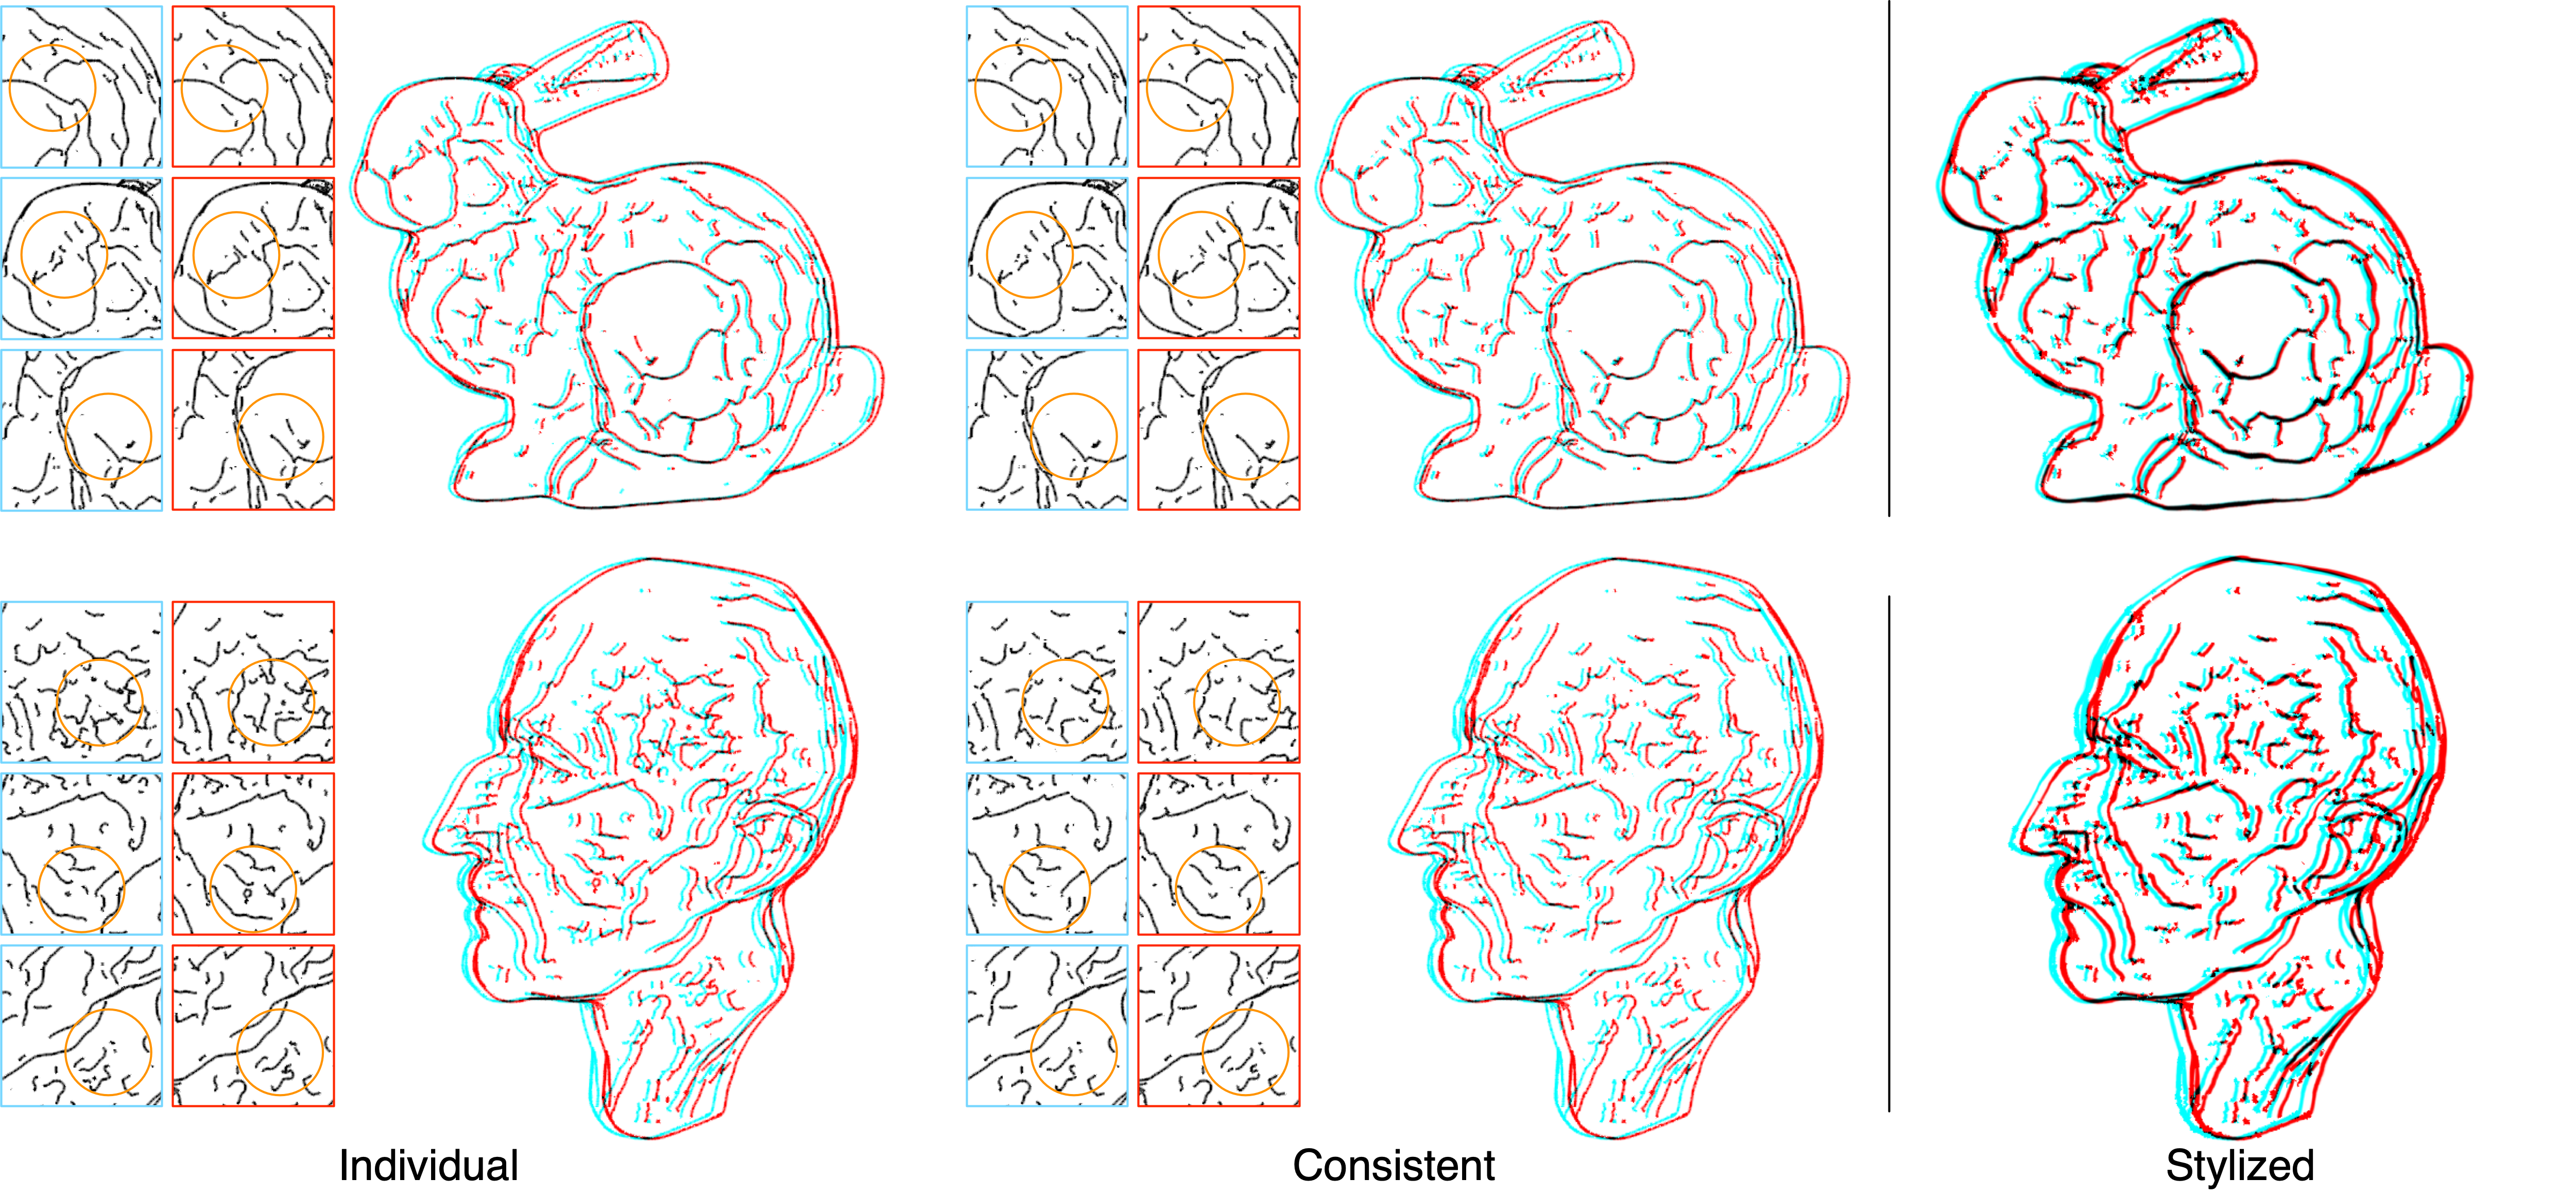
\includegraphics[width=\linewidth]{basic}
    \caption{\label{fig:basic}
    用直接方法生成的双目图像和用本文提出的方法生成的双目图像的对比。推荐使用三维红蓝眼镜来获得更好的观察体验。最右边展示的是在\stc{}结果上进行进一步风格化的结果。使用的三维模型来自DeCarlo等人的工作\cite{DFRS03}。
    }
\end{figure*}
  
\begin{figure*}[!t]
    \centering
    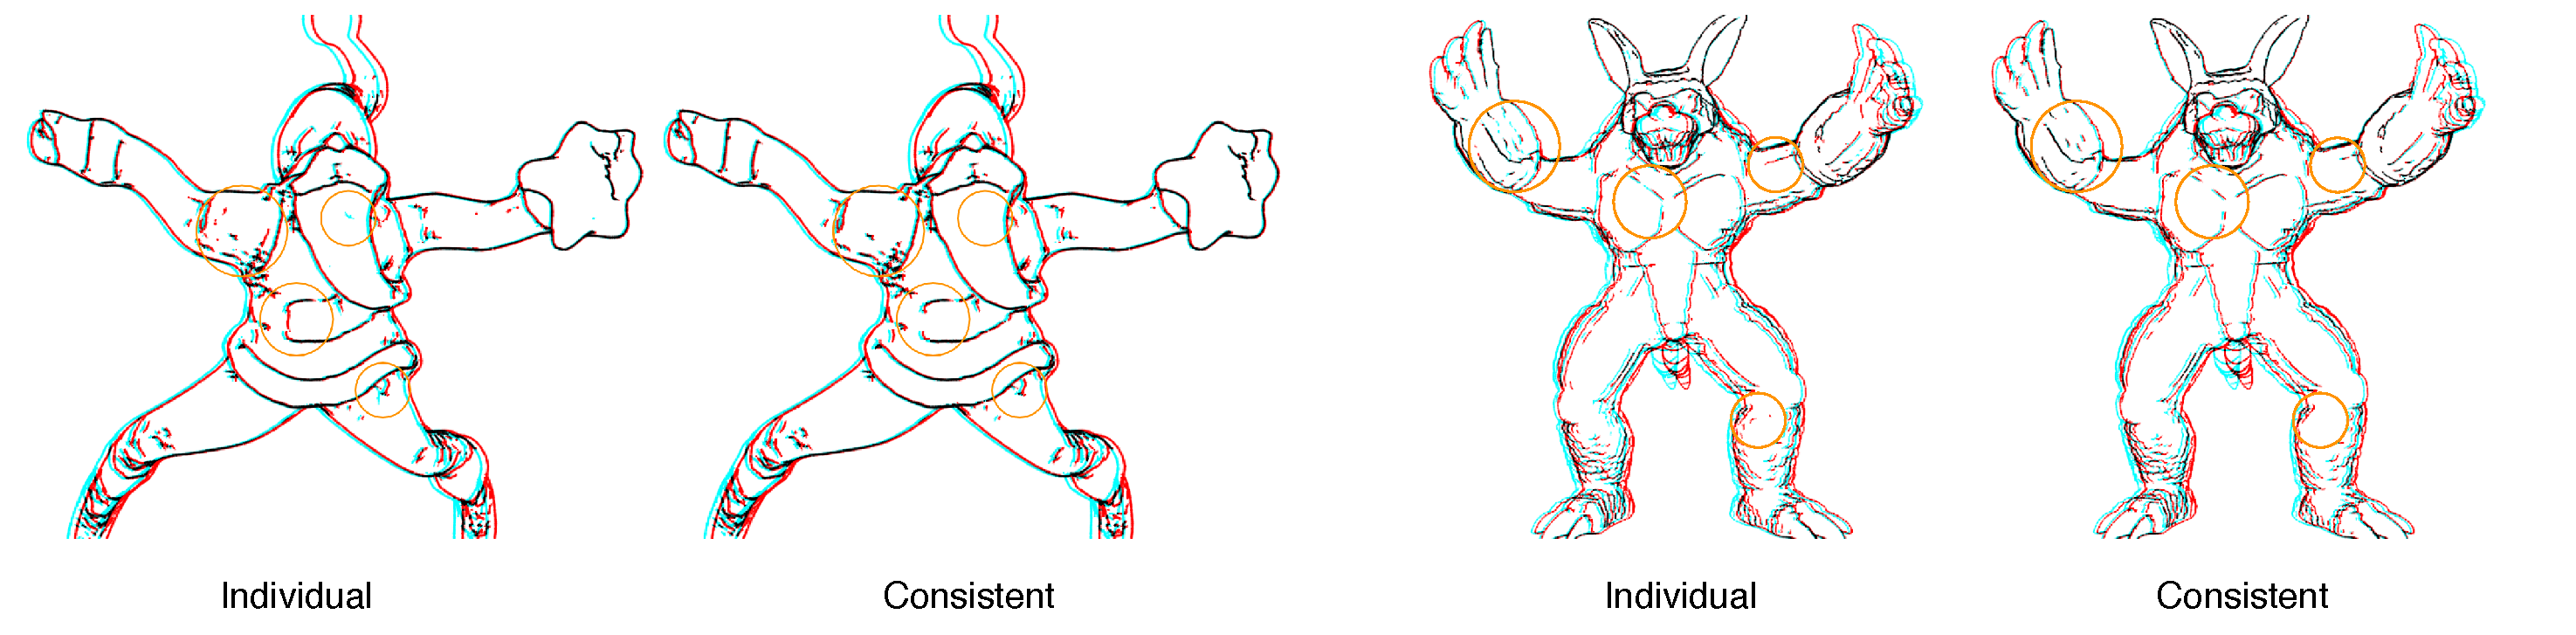
\includegraphics[width=\linewidth]{more}
    \caption{\label{fig:more}
    更多用直接方法生成的双目图像和用本文提出的方法生成的双目图像的对比。
    }
\end{figure*}

首先,为了评估本文提出的方法的质量,本文展示了用直接方法生成的双目图像和用本文提出的方法生成的双目图像的对比(\autoref{fig:basic}, \autoref{fig:more})。图中有部分放大的区域,从这些区域可以看出更细节的对比。从这些结果可以看出,本文提出的方法有效地消除了不是\stc{}那些\con{}和\scon{}。

\begin{figure*}[!t]
    \centering
    \includegraphics[width=\linewidth]{comparison}
    \caption{\label{fig:comparison}
    前人工作\cite{kim2013stereoscopic,bukenberger2018stereo}所展示的结果和本文方法所生成的结果的对比。由于无法获取前人工作所展示结果使用的一些绘制参数,所以本文方法生成的结果是通过手动调节参数来尽量使得艺术效果上尽量一致。但是由于使用的模型或者轮廓线绘制算法实现上的差异,部分细节仍会有所出入。天马的图像是根据深度对笔画宽度进行风格化的结果。使用的模型来自IMATI和CNR的AIM@SHAPE-VISIONAIR Shape Repository\cite{INR04}。}
\end{figure*}  

其次,为了进一步验证本文提出的方法的有效性,本文在\autoref{fig:comparison}中展示了前人工作\cite{kim2013stereoscopic,bukenberger2018stereo}所展示的结果和本文方法所生成的结果的对比。由于无法获取前人工作所展示的结果使用的一些绘制参数,所以本文方法生成的结果是通过手动调节参数来尽量使得艺术效果上尽量一致。从这些结果可以看出,尽管细节上有些许差异,本文提出的方法能够实现立体一致程度与前人方法所实现的程度基本一致。

\begin{figure}[!t]
    \centering
    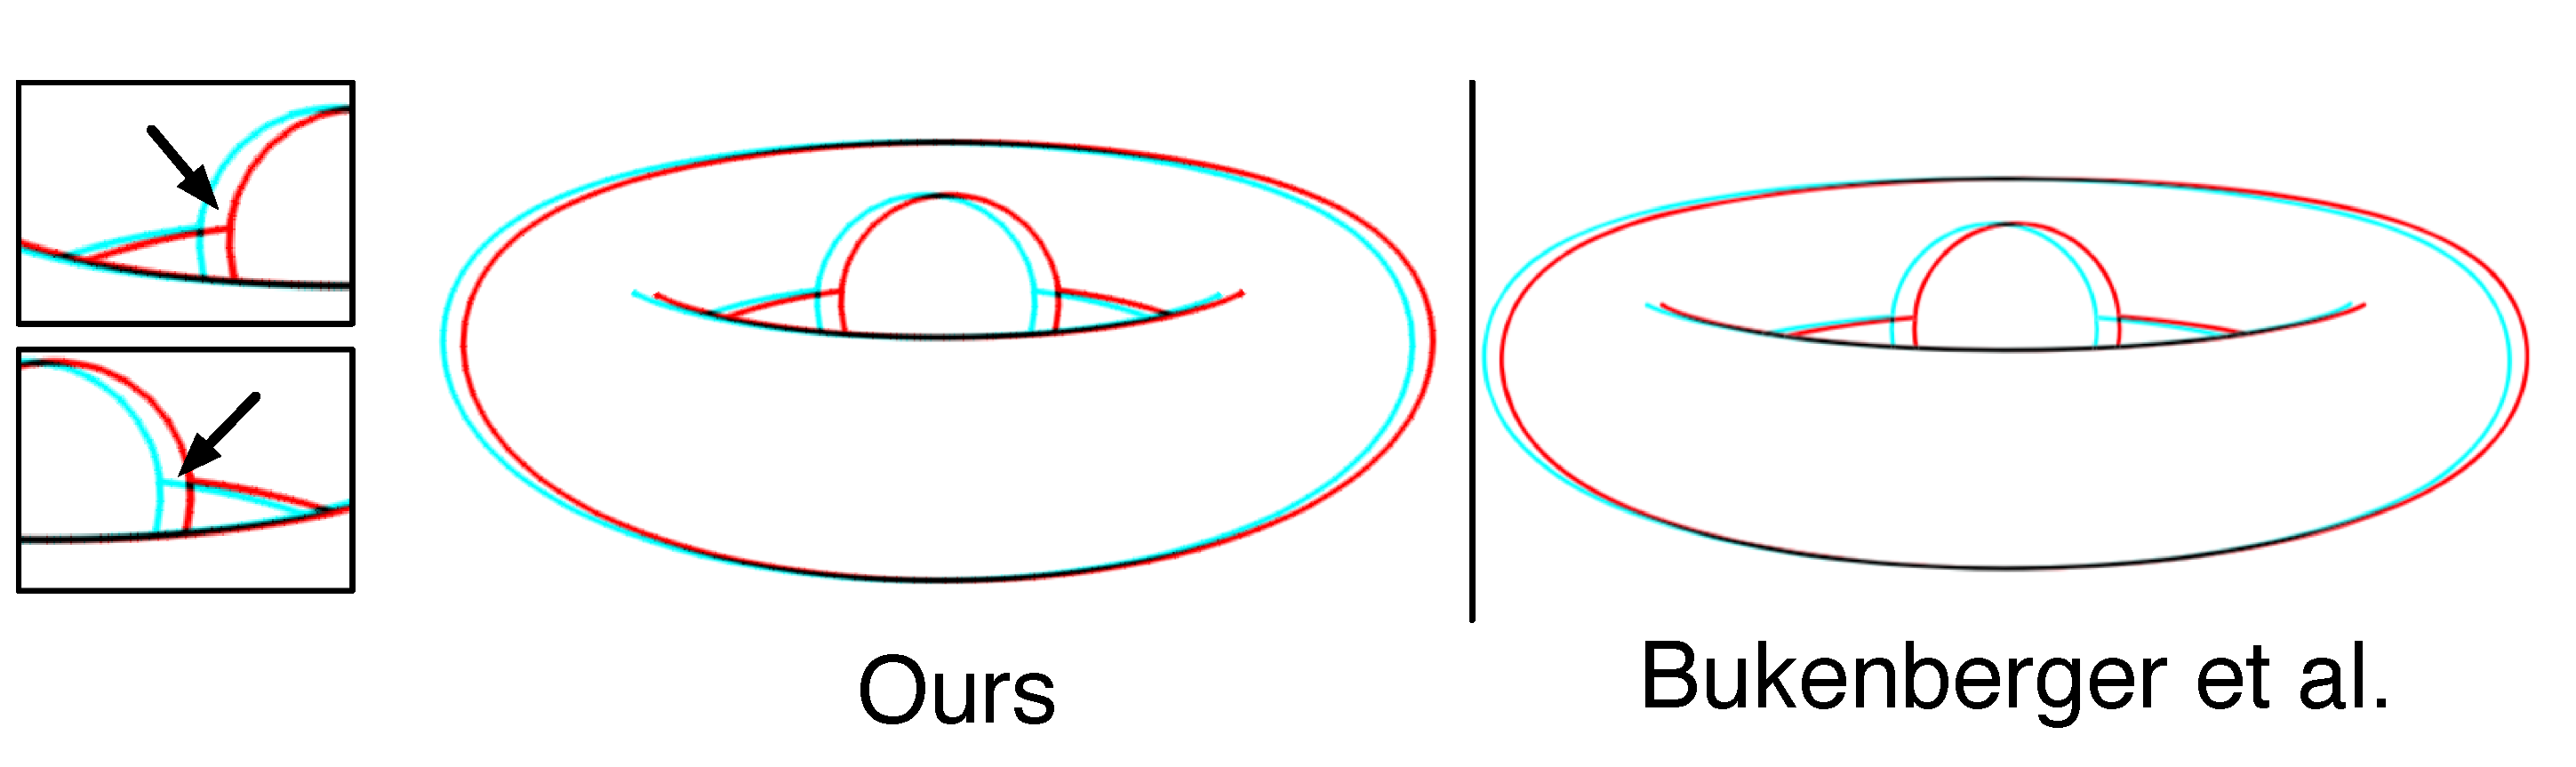
\includegraphics[width=\linewidth]{hidden}
    \caption{\label{fig:hidden}
    在线条被遮挡的情况下的匹配。使用了方框和箭头来指出被遮挡的线条。右边展示了来自于另一工作\cite{bukenberger2018stereo}的相似结果作为对比。}
\end{figure}

尽管本文提出的方法只在图像空间进行处理,但是被遮挡的线条也无须任何特别处理就能被正确地匹配,因为被遮挡的轮廓点也被存储在了\ppll{}之中。\autoref{fig:hidden}展示了一个在存在遮挡的情况下用本文设计的方法生成的和前人工作中的结果相似的的结果。

由于本文提出的方法不依赖于任何的预计算,所以本文提出的方法支持变化视点下的动态场景,并且支持实时的参数调节。

\section{效率对比}

\begin{table}[!t]
    \renewcommand{\arraystretch}{1.3}
    \centering
  \begin{threeparttable}
    \caption{示例场景的效率数据$^1$}
    \label{tab:performance}
    %\scriptsize
    % \small
    \centering
    \begin{tabular}{c|cc|ccc|c}
    \hline
    \multirow{2}{*}{场景} & \multirow{2}{*}{顶点数} & \multirow{2}{*}{面片数} & \multicolumn{4}{c}{效率 (ms / FPS)} \\
    \cline{4-7}
    & & & I & II & III & Total \\
    \hline
    Bunny (\autoref{fig:basic}) & 35947 & 69451 & {2.2} & {2.1} & {0.3} & {4.9/204.0} \\
    Max Planck (\autoref{fig:basic}) & 49132 & 98260 & {2.5} & {3.0} & {0.5} & {6.3/158.7} \\
    Homer (\autoref{fig:comparison}) & 5103 & 10202 & {0.6} & {2.3} & {0.1} & {3.2/312.5} \\
    Pegasus (\autoref{fig:comparison}) & 63544 & 127095 & {3.7} & {2.7} & {0.7} & {7.4/135.1} \\
    \hline
    \end{tabular}
    \begin{tablenotes}
      \item $^1$ 从左到右分别是:场景,顶点数,面片数以及阶段I,阶段II,阶段III以及整体的效率数据。数据是在关闭轮廓线风格化的情况下记录的。
    \end{tablenotes}
  \end{threeparttable}
\end{table}

本文使用PC平台上的OpenGL 4.6实现所展示的\stc{}轮廓线绘制系统,所使用的CPU为Intel Xeon E3,GPU为NVIDIA GeForce RTX 2080 Ti。当个绘制图像的分辨率为1024$\times$768。

\autoref{tab:performance}展示了绘制\autoref{fig:basic}和\autoref{fig:comparison}所示结果的效率。需要指出的是,这些时间数据是在关闭轮廓线风格化的情况下记录的。在对比之下可以看出,\citeauthor{kim2013stereoscopic}实现的系统\cite{kim2013stereoscopic}在使用GPU并且顶点数量达到30,000的情况下效率是每秒3帧。\citeauthor{bukenberger2018stereo}在他们的工作中实现了一个更高效的系统\cite{bukenberger2018stereo},在使用CPU并且面片数达到20,000的情况下能够达到每秒24帧的效率,但是在他们的工作中没有提及使用GPU的情况。然而,这样的效率是他们在没有正确考虑视点相关的遮挡的情况下得到的。在他们的方法中,即使对于像犹他茶壶(Utah Teapot)这样只有2464面片的小模型,完整考虑视点相关遮挡所需要的视图(view graph)算法也需要消耗0.25秒,而对于像斯坦福兔子(Stanford Bunny)这样较大的模型则需要将近5秒。与上述前人的方法相比,本文提出的方法能够以更高的效率实现正确的\stc{}轮廓线绘制。

\section{方法限制与展望}

尽管本文提出的方法能够实现实时的\stc{}轮廓点绘制,但还存在一些限制。首先,使用物体的索引来排除错误匹配的方法在错误匹配来自于同一个物体时会失效。一个更可靠的用于排除错误匹配的方法还有待开发。其次,在本文的讨论中还没有对轮廓线的时序一致性(temporal coherency)进行考虑。因此,在视频结果中会出现轮廓线的闪烁的情况,在轮廓线启用风格化的情况下这种问题会更加明显。出现这个问题的根源在于立体一致性和时序一致性之间会存在冲突,如果想要保证立体一致性,则需要根据物体的几何特征进行轮廓线的风格化,而如果想要保证时序一致性,那么需要传递风格化参数。因此,一个能够支持时序一致性的方法是未来研究的一个很有价值的目标。